% Adjust these for the path of the theme and its graphics, relative to this file
%\usepackage{beamerthemeFalmouthGamesAcademy}
\usepackage{../../beamerthemeFalmouthGamesAcademy}
\usepackage{multimedia}
\graphicspath{ {../../} }

% Default language for code listings
\lstset{language=C++,
        morekeywords={each,in,nullptr}
}

% From http://blog.virtualglobebook.com/2011/02/syntax-highlighting-c-and-glsl-source.html

\lstdefinelanguage{GLSL}
{
sensitive=true,
morekeywords=[1]{
attribute, const, uniform, varying,
layout, centroid, flat, smooth,
noperspective, break, continue, do,
for, while, switch, case, default, if,
else, in, out, inout, float, int, void,
bool, true, false, invariant, discard,
return, mat2, mat3, mat4, mat2x2, mat2x3,
mat2x4, mat3x2, mat3x3, mat3x4, mat4x2,
mat4x3, mat4x4, vec2, vec3, vec4, ivec2,
ivec3, ivec4, bvec2, bvec3, bvec4, uint,
uvec2, uvec3, uvec4, lowp, mediump, highp,
precision, sampler1D, sampler2D, sampler3D,
samplerCube, sampler1DShadow,
sampler2DShadow, samplerCubeShadow,
sampler1DArray, sampler2DArray,
sampler1DArrayShadow, sampler2DArrayShadow,
isampler1D, isampler2D, isampler3D,
isamplerCube, isampler1DArray,
isampler2DArray, usampler1D, usampler2D,
usampler3D, usamplerCube, usampler1DArray,
usampler2DArray, sampler2DRect,
sampler2DRectShadow, isampler2DRect,
usampler2DRect, samplerBuffer,
isamplerBuffer, usamplerBuffer, sampler2DMS,
isampler2DMS, usampler2DMS,
sampler2DMSArray, isampler2DMSArray,
usampler2DMSArray, struct},
morekeywords=[2]{
radians,degrees,sin,cos,tan,asin,acos,atan,
atan,sinh,cosh,tanh,asinh,acosh,atanh,pow,
exp,log,exp2,log2,sqrt,inversesqrt,abs,sign,
floor,trunc,round,roundEven,ceil,fract,mod,modf,
min,max,clamp,mix,step,smoothstep,isnan,isinf,
floatBitsToInt,floatBitsToUint,intBitsToFloat,
uintBitsToFloat,length,distance,dot,cross,
normalize,faceforward,reflect,refract,
matrixCompMult,outerProduct,transpose,
determinant,inverse,lessThan,lessThanEqual,
greaterThan,greaterThanEqual,equal,notEqual,
any,all,not,textureSize,texture,textureProj,
textureLod,textureOffset,texelFetch,
texelFetchOffset,textureProjOffset,
textureLodOffset,textureProjLod,
textureProjLodOffset,textureGrad,
textureGradOffset,textureProjGrad,
textureProjGradOffset,texture1D,texture1DProj,
texture1DProjLod,texture2D,texture2DProj,
texture2DLod,texture2DProjLod,texture3D,
texture3DProj,texture3DLod,texture3DProjLod,
textureCube,textureCubeLod,shadow1D,shadow2D,
shadow1DProj,shadow2DProj,shadow1DLod,
shadow2DLod,shadow1DProjLod,shadow2DProjLod,
dFdx,dFdy,fwidth,noise1,noise2,noise3,noise4,
EmitVertex,EndPrimitive},
morekeywords=[3]{
gl_VertexID,gl_InstanceID,gl_Position,
gl_PointSize,gl_ClipDistance,gl_PerVertex,
gl_Layer,gl_ClipVertex,gl_FragCoord,
gl_FrontFacing,gl_ClipDistance,gl_FragColor,
gl_FragData,gl_MaxDrawBuffers,gl_FragDepth,
gl_PointCoord,gl_PrimitiveID,
gl_MaxVertexAttribs,gl_MaxVertexUniformComponents,
gl_MaxVaryingFloats,gl_MaxVaryingComponents,
gl_MaxVertexOutputComponents,
gl_MaxGeometryInputComponents,
gl_MaxGeometryOutputComponents,
gl_MaxFragmentInputComponents,
gl_MaxVertexTextureImageUnits,
gl_MaxCombinedTextureImageUnits,
gl_MaxTextureImageUnits,
gl_MaxFragmentUniformComponents,
gl_MaxDrawBuffers,gl_MaxClipDistances,
gl_MaxGeometryTextureImageUnits,
gl_MaxGeometryOutputVertices,
gl_MaxGeometryOutputVertices,
gl_MaxGeometryTotalOutputComponents,
gl_MaxGeometryUniformComponents,
gl_MaxGeometryVaryingComponents,gl_DepthRange},
morecomment=[l]{//},
morecomment=[s]{/*}{*/},
morecomment=[l][keywordstyle4]{\#},
}


% For strikethrough effect
\usepackage[normalem]{ulem}
\usepackage{wasysym}

\usepackage{pdfpages}

% http://www.texample.net/tikz/examples/state-machine/
\usetikzlibrary{arrows,automata}

\newcommand{\modulecode}{COMP260}\newcommand{\moduletitle}{Distributed Systems}\newcommand{\sessionnumber}{5}

\begin{document}
\title{\sessionnumber: Getting Started with OpenGL}
\subtitle{\modulecode: \moduletitle}

\frame{\titlepage} 

\begin{frame}{Learning outcomes}
	By the end of this week, you should be able to:
	\begin{itemize}
		\item \textbf{Recall} alternative ways to represent mesh vertices in memory.
		\item \textbf{Apply} basic transforms using the GLM library.
		\item \textbf{Explain} the constituents of the model-view-projection matrix and how it can be used to create a first-person camera controller.
	\end{itemize}
\end{frame}

\begin{frame}{Agenda}
	\begin{itemize}
		\pause\item Lecture (async):
		\begin{itemize}
			\item \textbf{Compare} different ways to store vertex data in memory.
			\item \textbf{Review} the transforms required to display 3D objects on a 2D screen.
		\end{itemize}
		\pause\item Workshop (sync):
		\begin{itemize}
			\item \textbf{Adapt} our basic triangle implementation to draw meshes with multiple triangles efficiently.
			\item \textbf{Experiment} with creating transforms using GLM and using them to move objects and the camera.
		\end{itemize}
	\end{itemize}
\end{frame}

\part{Introducing OpenGL}
\frame{\partpage}

\begin{frame}{What is OpenGL?}
	\begin{itemize}
		\pause\item A \textbf{cross-language, cross-platform} API \textbf{specification} for rendering 2D and 3D vector graphics.
		\pause\item First released in 1992; current version: 4.6.
		\pause\item Major design changes in version 3.3/4.0 (2010):
		\begin{itemize}
			\pause\item Previously used \textbf{fixed function pipeline} with functionality hidden/abstracted: easy to use but inefficient.
			\pause\item Changed to \textbf{core-profile} mode: flexible and powerful, but more complex to learn.
			\pause\item Requires a greater understanding of what's actually happening.
		\end{itemize}
	\end{itemize}
\end{frame}

\begin{frame}{OpenGL as a specification}
	\begin{itemize}
		\pause\item Defines what the output of each function should be.
		\pause\item Libraries are (usually) implemented by the graphics card manufacturers:
		\begin{itemize}
			\pause\item \textbf{Core OpenGL (GL)}: functions prefixed with \lstinline{gl} to model an object view geometric primitives (point, line, polygon).
			\pause\item \textbf{OpenGL Utility Library (GLU)}:  functions prefixed with \lstinline{glu} to extend the core library.
			\pause\item \textbf{OpenGL Utilities Toolkit (GLUT)}: functions prefixed with \lstinline{glut} to interact with the operating system (e.g. handling input).
			\pause\item \textbf{OpenGL Extension Wrangler Library (GLEW)}: cross-platform C/C++ extension loading library.
		\end{itemize}
	\end{itemize}
\end{frame}

\begin{frame}{OpenGL as a state machine}
	\begin{itemize}
		\pause\item OpenGL itself \textbf{does not} retain information about objects.
		\pause\item Uses the \textbf{context}, which stores a collection of variables to define how to render triangles.	
		\pause\item To change a portion of the image by default requires \textbf{clearing} and \textbf{redrawing} the whole screen.
		\pause\item Change the state by \textbf{setting options} (e.g. draw mode) and \textbf{manipulating buffers}.
	\end{itemize}
\end{frame}

\begin{frame}{SDL and OpenGL}
	\begin{itemize}
		\pause\item OpenGL only handles rendering of graphics.
		\pause\item We need something else to handle windows, events, audio etc.
		\pause\item We will use \textbf{SDL} (which you have used before, including in COMP270).
	\end{itemize}
\end{frame}


\part{Shaders}
\frame{\partpage}

\begin{frame}{Recap: processing pixels}
	\begin{columns}
		\begin{column}{0.5\textwidth}
			\begin{center}
				\pause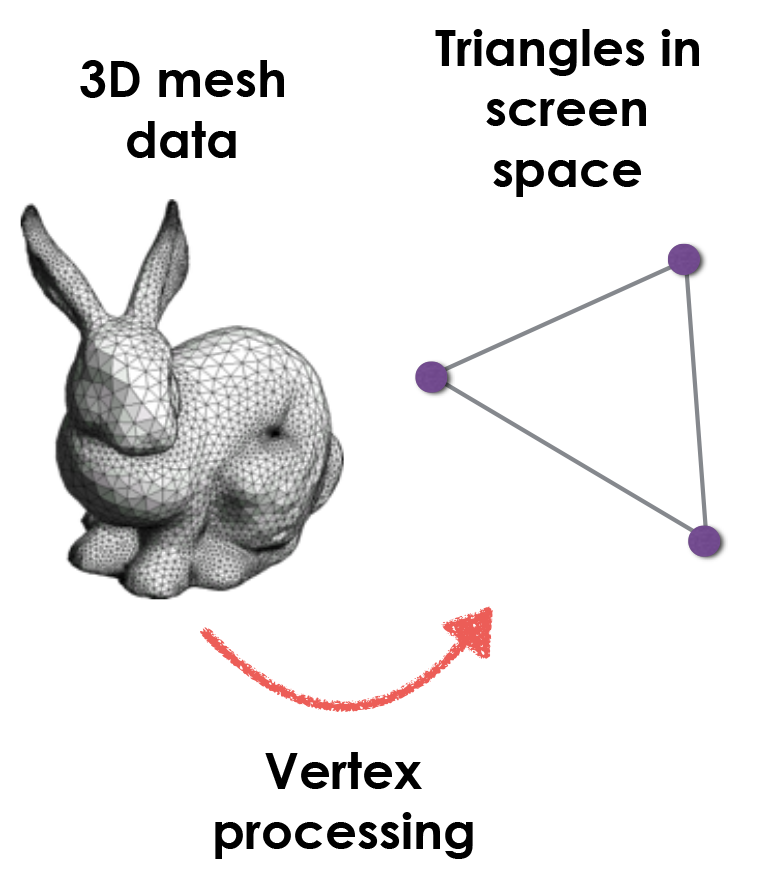
\includegraphics[height=0.85\textwidth]{vertex_processing}\\
			\end{center}
			Vertex processor \textbf{transforms} vertices and \textbf{projects} them into 2D screen space.
		\end{column}
		\begin{column}{0.5\textwidth}
			\begin{center}
				\pause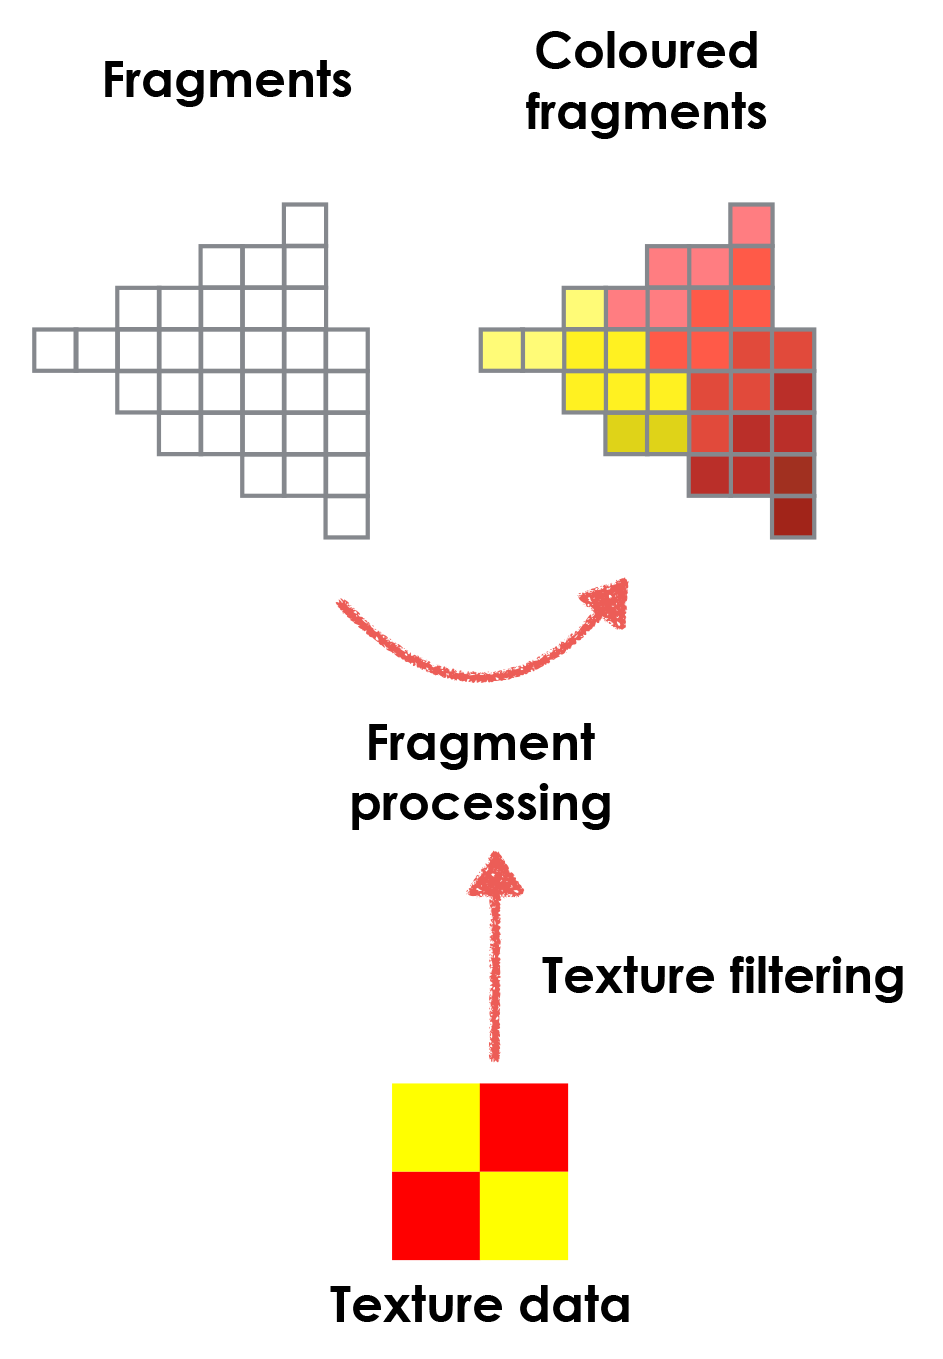
\includegraphics[height=0.85\textwidth]{fragment_processing}\\
			\end{center}
			Fragment processor determines the \textbf{colour} of each fragment covered by the triangle.
		\end{column}
	\end{columns}
\end{frame}

\begin{frame}{Vertex and fragment shaders}
	\begin{itemize}
		\pause\item The vertex processor and fragment processor are \textbf{programmable}
		\pause\item Programs for these units are called \textbf{shaders}
		\pause\item \textbf{Vertex shader}: responsible for geometric transformations, deformations, and projection
		\pause\item \textbf{Fragment shader}: responsible for the visual appearance of the surface
		\pause\item Vertex shader and fragment shader are separate programs,
			but the vertex shader can pass arbitrary values through to the fragment shader
	\end{itemize}
\end{frame}

\begin{frame}{Interpolation}
	\begin{columns}
		\begin{column}{0.5\textwidth}
			\begin{itemize}
				\pause\item The vertex shader sets a value for each vertex
				\pause\item So what is the value in the middle of the triangle?
				\pause\item The GPU \textbf{interpolates} the value across the triangle
			\end{itemize}
		\end{column}
		\begin{column}{0.45\textwidth}
			\pause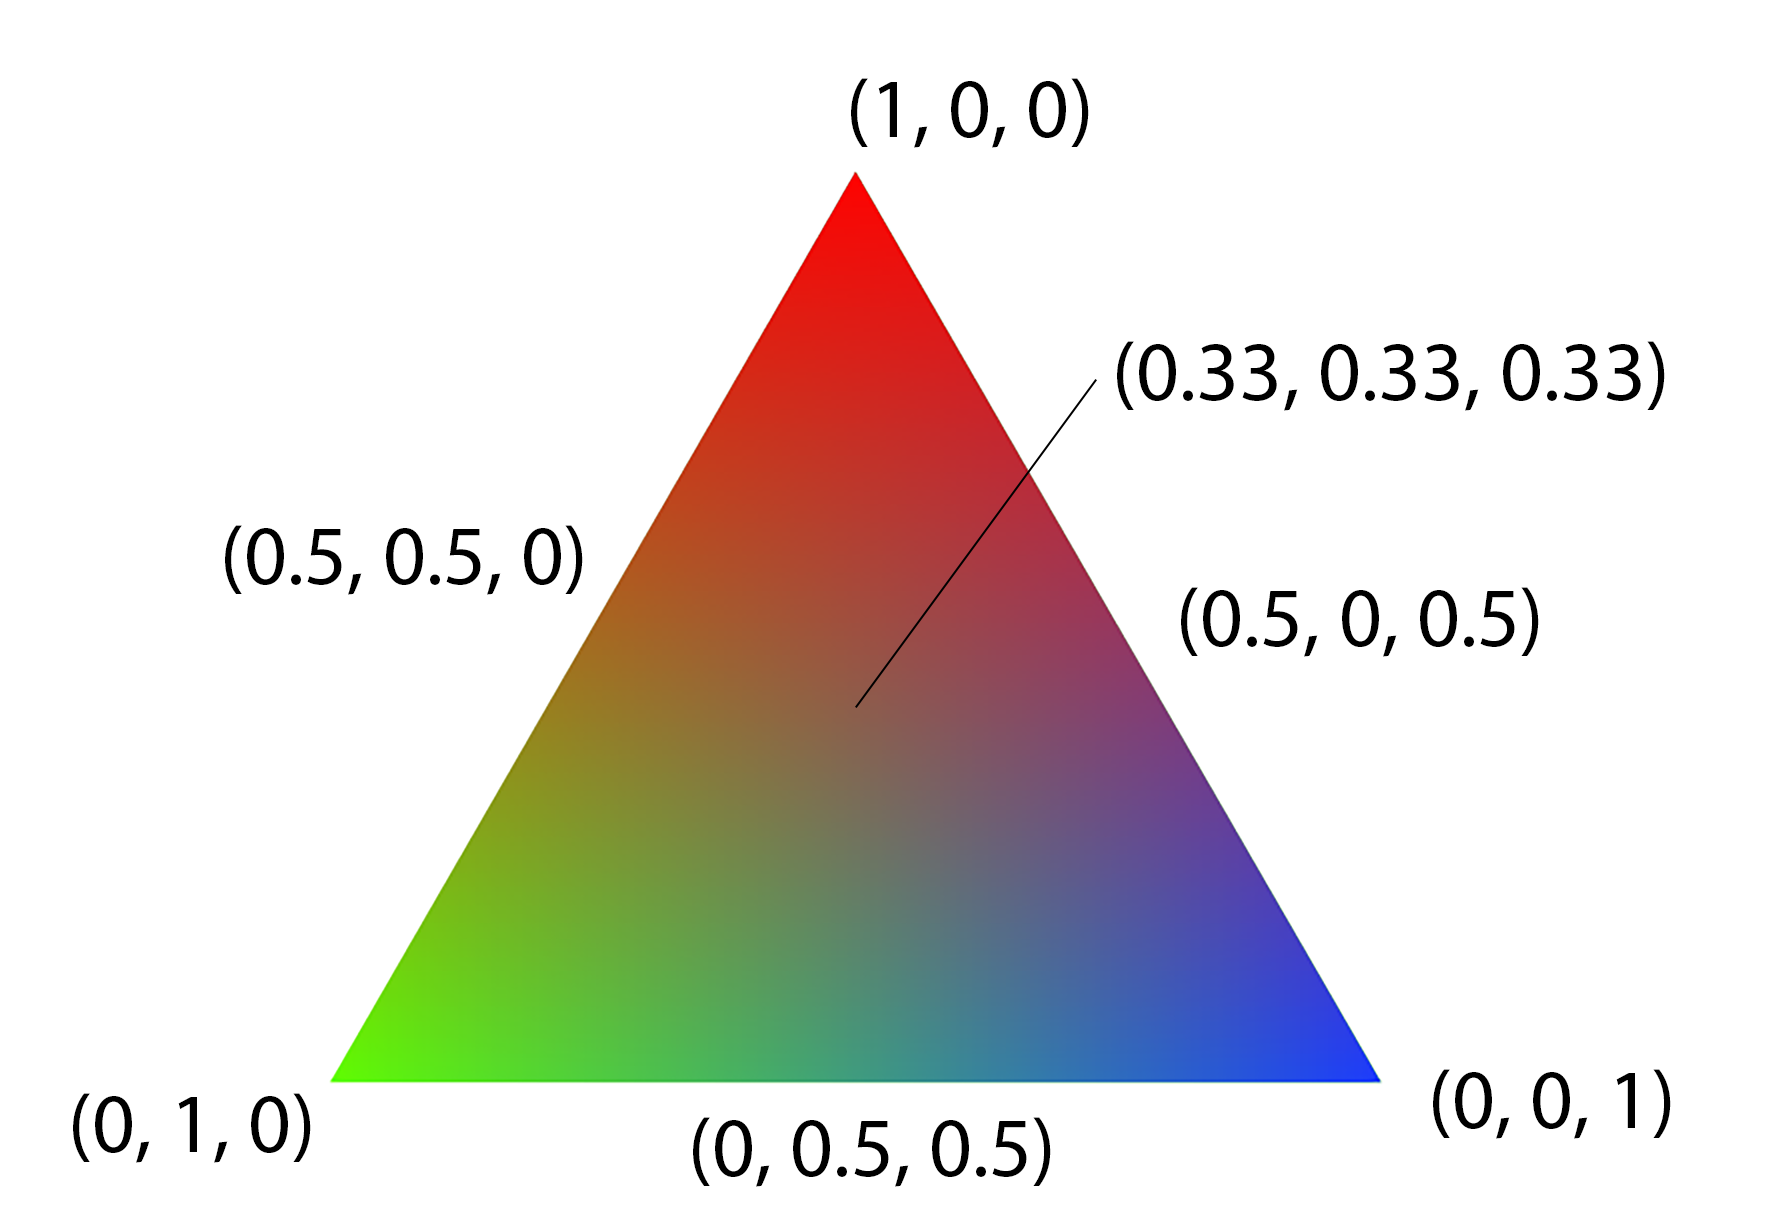
\includegraphics[width=\textwidth]{interpolation}
		\end{column}
	\end{columns}
\end{frame}

\begin{frame}{Next steps}
	\begin{itemize}
		\item \textbf{Review} the additional asynchronous material for more background on OpenGL and shaders/GLSL
		\item \textbf{Attend} the workshop to see how to use OpenGL with SDL to set up a scene and render it with shaders in GLSL
	\end{itemize}
\end{frame}

\end{document}

